\clearpage
\section{Evaluation of XDAQ framework}
\label{XDAQ-Mainchapter}

{\em XDAQ} \cite{XDAQ-wiki} is a data acquisition framework being developed for the {\em Compact Muon Solenoid} (CMS) experiment \cite{CMS-home} at CERN. The developers give the following mission statement:
''XDAQ is a middleware that eases the tasks of designing, 
programming and managing data acquisition applications by providing a simple, 
consistent and integrated distributed programming environment. 
The framework builds upon industrial standards, open protocols and libraries.''\cite{XDAQ-wiki}.
The XDAQ programming framework mainly consists in C++ classes
and namespaces, whereas also some JAVA based tools are applied.

Since the data acquisition of the CMS experiment is comparable in size with what is 
planned for CBM, XDAQ seems to be well suited as an example of such a system. Moreover,
the existing XDAQ system might be directly adaptable as framework for the first CBM
data acquisition test set up. Because of this, XDAQ was evaluated with respect to
the usability for CBM. XDAQ was installed on the standard gsi Linux,
and on the InfiniBand test cluster (section \ref{XDAQ-IB-install}).      
Here several tests were carried out using standard examples of the XDAQ release
(section \ref{XDAQ-tests}). For fast data transfer over the network is
crucial for CBM, a special emphasis was put on the data transport. 
Performance of different peer transport layers was measured by means of
a Roundtrip application (section \ref{RoundTripBasics}). The
applicability and the limits of InfiniBand transport within XDAQ framework 
was studied thoroughly. In
the course of this work, a new XDAQ peer transport module was developed
on top of the uDAPL library for InfiniBand   
(\ref{ptDAPL-Imp}).




\subsection{Installation on InfiniBand cluster}
\label{XDAQ-IB-install}
%Installation problems, patches for 64 bit, environment set up.
The first Installation attempts of XDAQ on the InfiniBand test machines encountered
some problems due to the 64 bit architecture, and differences of our Linux installation
(SuSe 9.3) to the CERN standard (Scientific Linux).
Thus some adjustments were necessary to build at least the basic
components.

The XDAQ framework is released as major 
packages {\em Coretools}, {\em Powerpack}, and {\em Worksuite}.
The {\em Worksuite} is specialized for CMS experiment hardware and
requires specific drivers and kernel mode compilation; it was mainly
excluded for these tests.

Concerning the 64 bit compatibility, at first 
the central Makefile parameters had to be modified to support
position independent code (option $-fPIC$). This allowed the
{\em Coretools} bundle to be build. For the XDAQ version of
November 2005, it was also necessary to disable some hardware oriented
modules of the {\em Powerpack}\footnote{XDAQ release of May2006 automatically 
disables these CMS specific parts now}.
Then the compilation seemed to be successfull.


However, some standard examples showed up strange behaviour on
runtime, e.g. the http port of the HyperDAQ web server
(see section\ref{HyperDAQtest}) was not ready while consuming 99\% cpu time; 
other operations lead to segmentation violations of the XDAQ executive.
Since this functionality was working well with a reference installation on standard GSI
linux (Debian 3.0, 32 bit), the sources were investigated concerning parts that
are not 64bit save.
In fact, modification of several places in the code with crucial pointer types 
let these problems disappear. These patches were reported to the XDAQ developer
community\footnote{This initiated advanced efforts of the developers to port the XDAQ code 
to 64 bit; meanwhile this has been achieved with the release of June 2006}.

This installation of November 2005 was applied for all general tests and
developments. In May 2005, the IB cluster installation was updated by the new
XDAQ developments ({\em Coretools 3.5.2}, {\em Powerpack 1.4.3}). 
Still our 64 bit corrections were necessary on top of this
release. Additionally, some other small compilation problems occured that
could be solved manually. 











%\clearpage
\subsection{XDAQ tests overview}
\label{XDAQ-tests}

%Here description of existing xdaq components that have been tested.
The installation of the {\em Coretools} and {\em Powerpack} components
on the IB cluster has been tested by means of standard examples as delivered
with the XDAQ distribution. Sourcecode and configuration files of the examples 
were put to a user working directory and slightly 
adjusted to the cluster environment. Additionally, some test applications 
were further developed and supplemented by other XDAQ features under
investigation.

Starting with the given {\em HelloWorld} example, it was already possible
to learn about the {\em XML} configuration files, and to explore the features 
of the {\bf Hyperdaq} web interface. 
Other tested examples covered:
\begin{compactitem}[$\bullet$]
 \item synchronous and asynchronous {\bf state machines} (\ref{StateMachineTest}); 
 \item multithreading with XDAQ {\bf workloop} mechanism;
 \item data import/export  by means of the XDAQ {\bf InfoSpace} (\ref{XDAQ-Monitor}); 
 \item monitoring of control variables with the XDAQ {\bf monitoring} tool (\ref{XDAQ-Monitor}); 
 \item command messaging with {\bf SOAP} protocol over the 
   {\bf peer transport http} layer (\ref{SOAPtest})
 \item data transport with {\bf I2O} protocol over the 
   {\bf peer transport TCP} (pt/tcp) layer (\ref{I2O}) 
\end{compactitem} 


Most of these features work together in the distributed XDAQ
{\em RoundTrip} benchmark application for data transport performance 
measurements. Therefore our advanced investigations were focused onto this 
example (i.e. the minor changed {\em MyRoundTrip}). 
 
The experiences with different XDAQ aspects from this work is described
in the following.

\subsection{Cluster configuration}
\label{XMLConfig}
% Here some details how xml configuration works: all nodes know all registered
% applications
XDAQ is designed to run many processes distributed over a data
acquisition cluster. The configuration of each process is set up by
an XML description schema \cite{XDAQ-XML}. Here certain hierarchical units are
defined by xml tags, such as {\em Partition}, {\em Context}, and  {\em Application}.
Additionally,  the {\em Endpoint} tag may define a network connection. 
Library modules can be specified by means of {\em Module} tag, they are
loaded automatically when activating the configuration.

The cluster itself may be divided into several {\em Partition}s; however,
XDAQ currently supports only one single partition.
All XDAQ applications of a {\em Partition} are grouped into different {\em Context}s 
on the network cluster. Each {\em Context} is usually identified by an URL, i.e. a
node name and a port number. All XDAQ {\em Application}s of the same 
{\em Context} will run as threads in one process on the node, controlled by the 
{\em XDAQ Executive} application. It is possible to pass individual default parameters to
each {\em Application} using a {\em properties} tag, including variable names 
as defined in the application code. 

At first, the default configuration for all contexts is loaded from the {\tt etc/profile.xml} file.
This defines at least the controlling {\em Executive} application environment, 
and the peer transport via http for external access of the node.
In addition, on startup of each XDAQ process, an individual configuration file
can be passed on the command line, e.g. {\tt xdaq.sh -c myconfiguration.xml}.
It is also possible to load a configuration file from the {\em HyperDAQ} web
interface (section \ref{HyperDAQtest}) into an {\em Executive} after the XDAQ start up.

It should be pointed out that this configuration file may be the same for all nodes
of the cluster. By means of the {\em Context} tag, each node will only apply the
settings for the own context, but is aware of the other contexts.
Thus each  {\em Executive} has a local registry of {\em all} applications in the network.
This is applied for addressing messages (section \ref{SOAPtest}), or
for browsing the cluster (section \ref{HyperDAQtest}).




\subsection{{\em HyperDAQ} web interface}
\label{HyperDAQtest}
%Feature description, xrelay controller, 

By default each XDAQ {\em Context} process (section \ref{XMLConfig}) runs a web server consisting
in the {\em HyperDAQ} application. The home page of this web server (Fig. \ref{fig:hyperdaq}) offers
a user interface for all known XDAQ applications in the cluster. It can
be viewed by any html browser at the {\em Context} http address and port number.
%{\tt http://depcp001.gsi.de:1972}. 
For security of the http access, XDAQ provides
the {\em XAccess} module which applies Basic http authentication and rejection of
unknown client addresses. Additionally, {\tt tinyproxy} is suggested as
lightweight http proxy to control access from outside a
private DAQ cluster \cite{XDAQ-wiki}.

\begin{figure}[htb]
\centering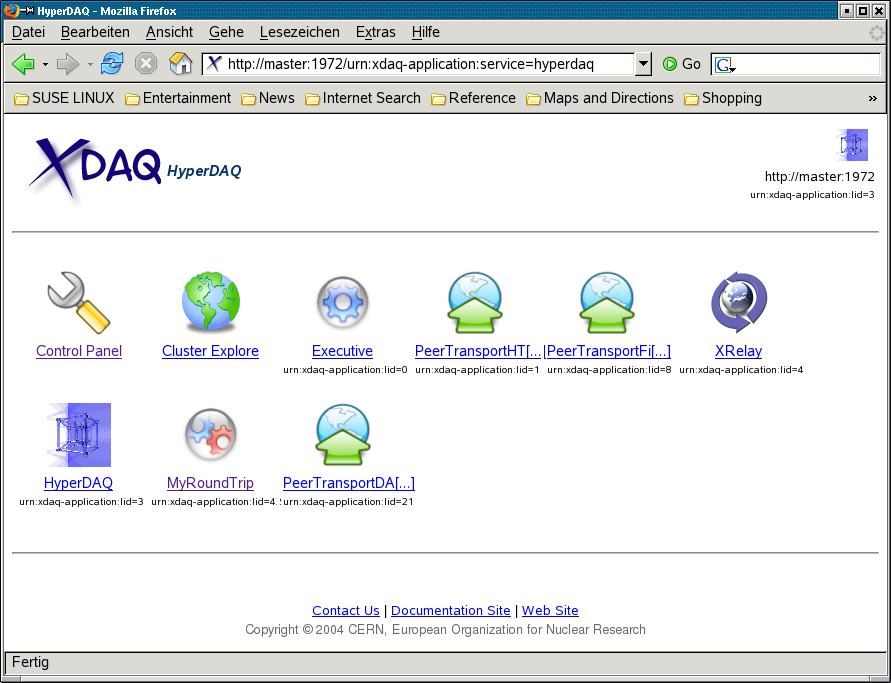
\includegraphics[angle=0,width=.8\textwidth]
{hyperdaq-screen.png}
\caption{A screenshot of the {\em HyperDAQ} web interface.}
\label{fig:hyperdaq}
\end{figure}





The properties of any application
may be inspected or even be changed via this web interface. Moreover, a
XDAQ application may be defined as {\em WebApplication}, with the possibility
to show an individual homepage when clicked from the {\em HyperDAQ}.
Using the XDAQ {\em xgi} library for cgi scripts, the developer may provide
a dynamic web-client user interface here. This feature was applied for theStateMachineTest
{\em state machine} (\ref{StateMachineTest}) and {\em MyRoundTrip} 
(\ref{RoundTripBasics}) examples, for instance.

Additionally, it is possible to send SOAP messages \cite{SOAP} to any
known XDAQ application by means of the {\em XRelay Controller} web interfaces, respectively. Like the {\em HyperDAQ}, the {\em XRelay Controller} is one of the XDAQ default applications running in each 
{\em Context} process.
The experiences with the {\em XRelay Controller} are described in section \ref{SOAPtest}.

Other features available from the {\em HyperDAQ} surface: 
\begin{compactitem}[$\bullet$]

\item the {\em Upload Application} form to start new applications on the
cluster by class name, id number, and library location;

\item the {\em Configure Executive} form to upload and apply a new xml configuration script;

\item the {\em Cluster Explore} tool that allows jumping to any other 
{\em HyperDAQ} server in the cluster;

\item lists of all loaded libraries on the {\em Display Modules} page

\item lists of all known applications with links to their properties and 
home pages on the  {\em Application Descriptors} page; 

\end{compactitem} 

To summarize, the {\em HyperDAQ} turned out to be very useful in this evaluation and development phase, as the tested applications could be inspected and
controlled easily. Except for the xml configuration file editor, no other
user interface was necessary for set-up and monitoring of the examples.
However, the existing web surfaces will most probably not be sufficient for
a data acquisition system ``in production''.


\subsection{State machines}
\label{StateMachineTest}
%Synchronous/asynchronous state machines. Description, work well.

A fundamental way to describe and control the behaviour of 
complex entities, e.g. data acquisition components, 
consists in the concept of the {\em Finite State Machine} (FSM) \cite{Wikipedia-Statemachine}.
The XDAQ framework already delivers some powerful classes
to realize such finite state machines.

The {\tt toolbox::fsm} package contains the {\bf FiniteStateMachine}
and {\bf AsynchronousFiniteStateMachine} classes; 
the latter using a dedicated workloop (thread) to process
the state transition functions in the background. Both classes allow
to configure arbitrarily the states and transition functions of the
state machine object: the user may define any kinds of states and their
transitions by text identifiers in the source code; any method of a user class 
may be bound to a specific state transition. XDAQ events with user defined
command names may be passed to an exisiting FSM to trigger 
state changes on runtime.

Additionally, the {\tt xgi} package offers the {\bf WSM} class as 
{\em web dialog state machine}. This alternative FSM implementation
is also user configurable at compile time, but has a web page GUI with
buttons to show and change the state.   
 
The data transport {\em RoundTrip} example (section \ref{RoundTripBasics}) uses
both FSM implementations in parallel. The web state machine is
just applied as user interface, whereas the FiniteStateMachine rules the
application state and may also be toggled by SOAP messages.  
Both state machines are always kept synchronized.

As predefined in the XDAQ examples, the states ``Halted'', ``Ready'', 
``Enabled'' are used here, with transition commands ``Configure'', ``Enable'',
and ``Halt'', respectively.  Since this kind of state machine is generally
applicable for many cases, the corresponding SOAP commands are already 
foreseen in the {XRelay} controller web interface (section \ref{SOAPtest}).
Therefore we kept this state machine definition as ``template'' 
to control all further test programs (sections \ref{RDMA-XDAQ}, 
\ref{RoundTripBasics}, \ref{ptDAPL-SendRec}). 
However, this functionality appears just as a suggestion and may be 
extended or fully redefined for a production system later on.

The XDAQ state machine concept seems powerful and flexible enough
to cope with all requirements for data acquisition set-up and control.
Issues that have not been covered yet in our investigations  are 
the performance (latency, CPU load) of state transitions, 
the reliability, and the stability, especially in case of large distributed 
systems. 


\subsection{Reading and monitoring of variables}
\label{XDAQ-Monitor}
%There is a monitor application for monitoring values. short!
Any data acquisiton system requires the possibility to monitor the state and
important values of the functional components, e.g. data rate, memory
and buffer consumption, etc. Though this task may be covered by independent,
full featured control systems, like EPICS \cite{EPICS}, or SMI++/DIM{\cite{DIM}},
XDAQ at least offers some mechanisms for monitoring of variables.

By the concept of the {\em Infospace} \cite{XDAQ-wiki}, it is possible to offer any value
for external readout by name. When a variable is requested from another
application, a user defined callback may ensure that its values are updated e.g. 
from a hardware component, or by calculation from other variables.

Moreover, XDAQ provides a default  {\em Monitor} application that may
request frequently variables from any other applications \cite{XDAQ-Monitor-wiki}. These variables
must be part of a known monitorable {\em Infospace}. 
By means of the {\tt mon:flashlists} tag in the XML configuration,
the variables to be monitored from any infospace are defined for
the {\em Monitor} application. Additionally, the {\tt mon:collectorsettings}
tag may specify the monitoring frequency, and properties for
recording a history of the values to a file.

Inspecting the monitored values from remote may be done via
a {\em Monitor CGI interface}. The {\em Monitor} application
example offers a xgi callback function that reacts on
a {\tt http::get} requests for a collected value from the flashlist. 
The result of such a variable retrieval may be a displayed as a table
in a web browser (when invoked from there), or may be printed
in the terminal (when invoked with {\tt curl} commandline tool \cite{CURL}).

The provided monitoring application example worked as intended for a small number of variables.
However, monitoring here always requires an {\em active} request of the visualizing client 
at the http server of the XDAQ {\em Executive} that runs the monitoring application.
This procedure might soon reach its limits when applied for a large number of
process variables on many nodes. Furthermore, the table 
display of the monitored variables in the requesting browser, as provided by the example, 
is very primitive compared to the possibilities of any slow control GUI.

Despite this, the example demonstrates the XDAQ possibilites for variable retrieval.
These can be applied for a more advanced monitoring system later on. For example, 
using the {\tt curl} library API \cite{CURL}, it would be possible to connect an independent EPICS 
{\em InputOutputController} process to the XDAQ http interface to fill process variables.
There are also ideas \cite{XDAQ-Monitor-wiki} to link the XDAQ variables via http or SOAP interfaces to National Instruments Labview  \cite{Labview} displays.
For the CMS experiment, XDAQ provides an interface to the LHC 
standard control system PVSS via SOAP messaging (section \ref{SOAPtest}) \cite{XDAQ-wiki}.



\subsection{Job Control}
\label{XDAQ-JobControl}
%There is a job control. What is it good for? possible starting point
%for real cluster control system\ldots?
The control of the data acquisition cluster not only requires to monitor
process variables, but also to change the state of the applications.
During the lifetime of the XDAQ {\em Executive}, this can be achieved by
passing commands via SOAP messages to the controlled XDAQ application, 
as described in \ref{SOAPtest}.

Moreover, to launch and cancel the {\em Executive} process itself,
a higher level control mechanism is necessary. This should be capable
of starting any operating system process on a machine of the DAQ cluster 
on initialization time; it may cancel any crashed process and restart it again
on the fly; finally, a regular shutdown of the DAQ processes should be
possible on remote request. One could also think of a supervising system
that may detect problems of the DAQ processes and recovers them automatically;
this ideas lead to systems like the  {\em ARMOR}s (\underline{A}daptive, 
\underline{R}econfigurable,
and \underline{M}obile objects for \underline{R}eliability), as 
proposed elsewhere \cite{Armor-paper}, \cite{Armor-survey}.

The XDAQ framework still does not provide such an elaborate system.
However, there is a {\em JobControl} application \cite{XDAQ-wiki} for starting and killing
any process from remote by means of SOAP requests (see \ref{SOAPtest}).
The {\em JobControl} runs within an independent, reserved XDAQ {\em Executive} process.
This may be launched before all other XDAQ processes, e.g. as a system service at Linux bootstrap time. 
Then the {\em JobControl} application can launch another XDAQ process with its own environment
that runs the real data acquisition applications. The {\em JobControl} can also kill the
other XDAQ process on request. 

There are several SOAP commands to initiate these actions from the controlling client:

\begin{description}

\item[executeCommand:] Start an executable on this machine. May define environment variables
and user settings. Note that any program may be invoked here, not only XDAQ processes.  

\item[killExec:] Kill an executable by id number

\item[killAll:] Kill all executables started by this job control 
 
 \end{description}

 
On our InfiniBand cluster, the {\em JobControl} has not been completely tested yet.
It seems a good idea though to provide a meta application for process control.
For a future DAQ production system, the {\em JobControl} concept could be developed
further to a semi-automatic node controller process. However, it still must
be investigated if there are other process controlling systems with similar or
even better properties.  
 

\subsection{SOAP messaging}
\label{SOAPtest}
%Here controller application that sends/receives configure messages to all exisiting xdaq applications in cluster.
XDAQ uses the {\em Simple Object Access Protocol} SOAP \cite{SOAP} to exchange 
commands and messages between the applications. From the 
{\em XRelay Controller} web interface (\ref{HyperDAQtest}), e.g., it is possible to submit interactively a SOAP  message to any registered application 
in the cluster.

\begin{figure}[htb]
\centering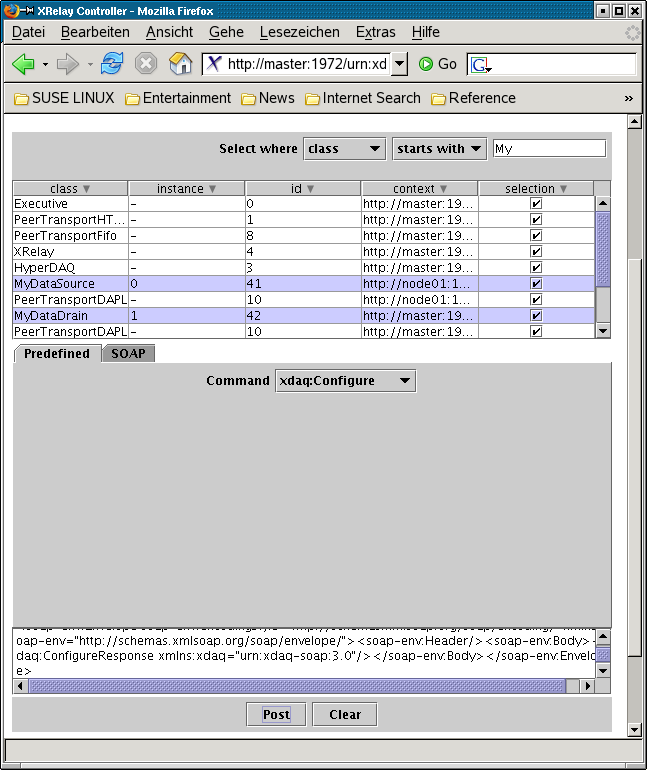
\includegraphics[angle=0,width=.8\textwidth]
{xrelay-screen.png}
\caption{A screenshot of the {\em XRelay Controller} web interface.}
\label{fig:xrelay}
\end{figure}


By means of a JAVA based web GUI (Fig. \ref{fig:xrelay}), the {\em XRelay Controller}  displays 
all known applications and allows to select the message receiver, or filter
multiple receivers by name pattern, respectively. Thus multiple 
receivers can be addressed by one click. 
Some default messages as standard commands for the XDAQ state 
machine examples (e.g. ``Configure'', ``Enable'', ``Halt'', ``Suspend'', 
``Resume'',  
see \ref{StateMachineTest}) 
can be selected by mouse from a list.
Besides these predefined messages, the web interface allows to edit the SOAP
statements to be send. The SOAP response message as returned from the
receiver will be displayed.


The {\em XRelay Controller} GUI  was used for most of our test as a 
simple command interface, 
since  the receiver actions for these commands are fully user defined. 
The web user interface turned out to be suitable for a limited number 
of applications,  but is supposed not to be sufficient as a ``real'' 
controls system.

However, by means of the {\em xoap} library XDAQ offers a powerful C++ API for 
inter-application SOAP messaging. 
This could be used as interface for more advanced controls application. 
A cluster set-up controller application would be possible
that communicates by SOAP messages with all other registered
applications. A first simple test program {\em MyController} has been developed 
to gain 
experiences with the API. Using the XDAQ application registry and SOAP 
messaging, it was possible to detect all running XDAQ user applications 
from the controller, and to initialize them.  

 
\subsection{I20 messaging}
\label{I2O}
% here i2o experiences and summary
The XDAQ concept clearly separates the messaging protocol from the
transport implementation layer. The user code just posts
messages of a certain format to a target application, or receives other 
messages  in dedicated callback functions, respectively. The transport
in between the XDAQ application is meant to be transparent for the user code.
In fact, just by changing the peer transport definition in the 
XDAQ cluster configuration file, the same
application may use different peer transport implementations without 
the need to recompile the code. Fig. \ref{fig:i2omessaging} illustrates
the XDAQ messaging architecture.

\begin{figure}[htb]
\centering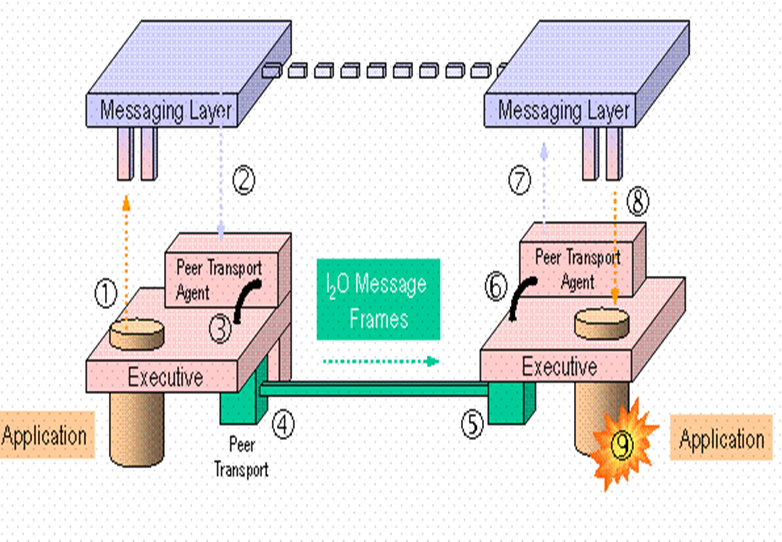
\includegraphics[angle=0,width=.8\textwidth]
{xdaqmessaging2.png}
\caption{{\em I2O} messaging and peer transport layers \cite{XDAQ-wiki}.}
\label{fig:i2omessaging}
\end{figure}



For exchange of commands and status information, XDAQ applies SOAP \cite{SOAP} 
as protocol,  while the transport over the network is handled by the 
{\em PeerTransportHTTP} library here (see section \ref{SOAPtest}).

For the experimental data stream, XDAQ chose the {\em Intelligent Input Output} 
({\bf I2O}) \cite{I2O} as standard binary message format.
The I2O structure features a standard data header, containing numerical sender
and receiver information, fields for certain flags, and a variable function code
number to indicate which actions should be done on receiving this message.
The data field appended to the header is arbitrarily definable by the user.
The XDAQ {\tt i2o} and {\tt i2o:utils} namespaces deliver methods to
format I2O messages, or to bind a user method as callback function
to an incoming I2O message, respectively. The substructure of the
I2O message and the reaction on receiving a message are free for the
user.

As default peer transport implementations for the I2O, XDAQ offers the 
{\bf Peer Transport FIFO} for  data exchange within one node, and the
{\bf Peer Transport TCP} to apply tcp/ip transport in between cluster
nodes. Additionally, an asynchronous peer transport for tcp/ip exists, 
{\bf Peer Transport ATCP}, that uses multithreaded senders to gain
performance.

\subsection{The {\em RoundTrip} benchmark}
\label{RoundTripBasics}
%Description of Roundtrip example, what is measured, theory of my
%figures of merit ($c$, $\tau_{0}$).

Most tests on the I2O messaging were run with the standard data 
{\em RoundTrip} example as distributed from XDAQ release. This
example was further adjusted (and renamed to {\em MyRoundTrip}), 
since special tests  in the course of the peer transport for 
uDAPL developments (section \ref{ptDAPL-Imp}) were necessary.

{\bf Functionality:}
The round trip benchmark is implemented into one class {\em MyRoundTrip},
that runs both as sender and receiver application on different nodes. The
different sender/receiver roles are identified by 
the instance number in the xml configuration file. The test run is
controlled by finite state machines (section \ref{StateMachineTest}) that
are either triggered from SOAP messages, or by the GUI elements of the
local web state machine.

The {\em Configure} command will execute method {\tt ConfigureAction()} which
will allocate memory and retrieve the handle for the connection from
the environement setup.
On {\em Enable} command, the sender will post a number of I2O message 
frames to the receiver. The {\em pipeLine} parameter in the setup will
define how many frames are initially send.

The {\tt token()} method both on sender and receiver side is bound as a
callback to the type of I2O message as defined for this test.
The receiver will execute this method for each message arriving from
the sender. To realise the round trip, the {\tt token()} will just exchange
sender and receiver addresses in the message header, and post the same
message frame back to the original sender. Thus the same messages are
travelling to and fro between both {\tt token()} functions, once the
benchmark has been started.

Additionally, the original sender will use the XDAQ {\em toolbox::PerformanceMeter} object to evaluate time and bandwith for each transfer, respectively. 
The size of the transferred frames is increased systematically during the
benchmark, with ranges and intervalls as user defined 
in the XDAQ configuration file.
All measurements are recorded into a measurement history map and are
displayed on the MyRoundTrip web appplication ``home page''. These results can
be viewed and stored from any web browser via the {\em HyperDAQ} interface 
(see \ref{HyperDAQtest}). 



{\bf Relation between transfer time and bandwidth}
The bandwidth $B$ as calculated from xdaq ratemeter is calculated from the current package size $P$, and from the total package transfer time $\tau$ :
\begin{equation}
\label{eq-bpdef}
B(P) = {\genfrac{}{}{}{}{P} {\tau}}
\end{equation}

In the web display of the RoundTrip benchmark, the term ``latency'' is 
used for $\tau$. 
It should be pointed out that this value in fact means the complete
time between initiating the package send (using the {\em postFrame} method), 
and the arrival of the package in the bound i2o callback function 
in the receiver process.

When plotting $\tau$ as function of package size $P$, one observes that
the transfer time seems to be 
linearly growing with package size for larger packages:

 \begin{equation}
\label{eq-dTaudP}
{\genfrac{}{}{}{}{d\tau} {dP}} = c
\end{equation}
with $c$ being a constant in units $\mu$s/kB. 

This equivalents: 


\begin{equation}
\label{eq-taup}
\tau(P) = c \cdot P + \tau_{0} 
\end{equation}



Combining (eq. \ref{eq-bpdef}) and (eq. \ref{eq-taup}), 
one gets for the bandwidth versus package size:
\begin{equation}
\label{eq-bp}
B(P) = {\genfrac{}{}{}{}{1}{{\left(c+{\tau_{0}/P}\right)}}}
\end{equation}


The bandwidth vs. package size can then be parametrized by two constants: the minimum latency $\tau_{0}$, and the slope of the latency increase with package 
size $c$.
 
For big packages $P \to\infty$, the bandwidth converges against the 
inverse latency slope:
\begin{equation}
\label{eq-bp-infty}
B(P)_{P \to\infty} = {\genfrac{}{}{}{}{1} {c}} 
\end{equation}

Thus, the latency slope $c$  reflects directly the limits of the transport layer (network) and is not due to performance loss of the messaging framework.
This is actually observed in the measurements 
(sections  \ref{RoundTripTestTCP}, \ref{RDMA-XDAQ}, 
\ref{ptDAPL-RoundTrip}, \ref{ptDAPL-SendRec}, \ref{ptDAPL-SendMultRec}, 
and \ref{ptDAPL-MultSendRec}).




For small packages $ P\cdot c \ll \tau_{0}$, 
the slope of the bandwidth is approximately:

\begin{equation}
\label{eq-bp-zero}
{\genfrac{}{}{}{}{dB(P)}{ dP} }_{P \to\ 0}= {\genfrac{}{}{}{}{1}{\tau_{0}}} 
\end{equation}

thus only ruled by the minimum latency.


\subsection{Roundtrip benchmark for Peer Transport TCP}
\label{RoundTripTestTCP}
%Here native roundtrip benchmarks and results
\begin{figure}[htb]
\centering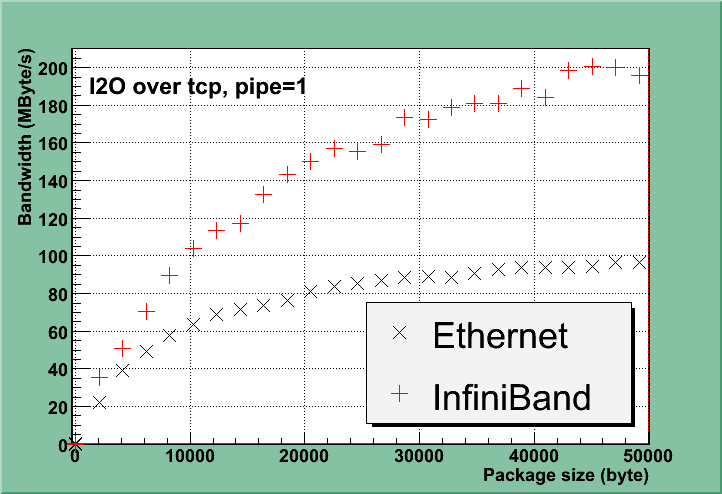
\includegraphics[angle=0,width=.8\textwidth]
{RoundtripTCP.png}
\caption{Bandwidth versus package size for peer transport tcp implementation,
compared between Ethernet and InfiniBand tcp stack.}
\label{fig:tcproundtripbw}
\end{figure}


At first, the roundtrip was performed with the plain tcp peer transport
between 2 nodes. It turned out that the decoupling between message and
protocol layer worked well for this example: the peer transport tcp
could switched on startup between Ethernet and InfiniBand networks just
by editing the configuration file. Moreover, peer transport tcp and atcp
could be exchanged as easily without changing the MyRoundTrip source codes.







As a typical result of these measurements, fig.\ref{fig:tcproundtripbw}
shows the bandwidth versus the frame size for tcp over ethernet, in
comparison with tcp over InfiniBand. The {pipeLine} length was set to 1 here,
i.~e. there was only one package being reflected between both applications.

As expected the InfiniBand shows 
a better performance. However, the theoretical limit of about $1$~Gbyte/s
was not achieved even for big packages.  
From a linear fit of (eq. \ref{eq-taup}) at the measured $\tau(P)$ data,
one gets figures of merit as presented in table \ref{tab-ether-ib-tcp}.



\begin{table}[htb]
\begin{center}

\begin{tabular}{|l|c|c|c|}\hline



Transport  & $\tau_{0} [\mu\mbox{s}]$ & $c [\mu\mbox{s}/\mbox{kByte}]$ & $B_{P\to\infty} [\mbox{MByte/s}]$ \\ \hline\hline

Ethernet & 67.7 & 8.52 & 117 \\ \hline
InfiniBand & 60.5 & 3.53 & 283 \\ \hline

\end{tabular}
\caption{Zero latency and maximum bandwidth as derived from fit 
(eq.\ref{eq-taup}) to $\tau(P)$ for {\em RoundTrip} measurements with
peer transport tcp.
\label{tab-ether-ib-tcp}}
\end{center}

\end{table}
 
Together with eq. \ref{eq-bp-infty}, the transport limit bandwidth for
the tcp stack of InfiniBand only achieves up to $0.3$~\mbox{Gbyte/s}.
Moreover, the minimum latency of $\approx 60~\mu\mbox{s}$ is also much worse than
the $\approx 5~\mu\mbox{s}$ as measured from the plain InfiniBand library transport
benchmarks.

Results of roundtrip measurements for the peer transport via uDAPL
imlementation are presented in section \ref{ptDAPL-RoundTrip}.  



\subsection{XDAQ Roundtrip for Remote DMA with uDAPL}
\label{RDMA-XDAQ}
%Short form: first attempt to combine both libs. Result is that they
%are compatible.
From the benchmark results (section \ref{RoundTripTestTCP}), 
the InfiniBand data transport within the XDAQ framework
requires a better peer transport layer than tcp/ip to reach
the network possibilities. The goal was to implement a XDAQ peer transport library
based on the uDAPL interface \ref{ptDAPL-Imp}. The C++ wrapper classes that
have been developed for the general InfiniBand tests
(section \ref{uDAPL-cpp}) should be applied for this purpose.


As a first test, the roundtrip benchmark as described in (section \ref{RoundTripBasics})
was modified in a way that the performance measurement and state machine 
controls were kept like before, but the data transport did {\em not} happen
by I2O messaging over the peer transport layer. Instead, the basic
uDAPL interface class (\ref{uDAPL-cpp}) was used directly.
It turned out that there was no conflict between XDAQ and uDAPL
libraries when compiled and executed togehter.





\begin{figure}[htb]
\centering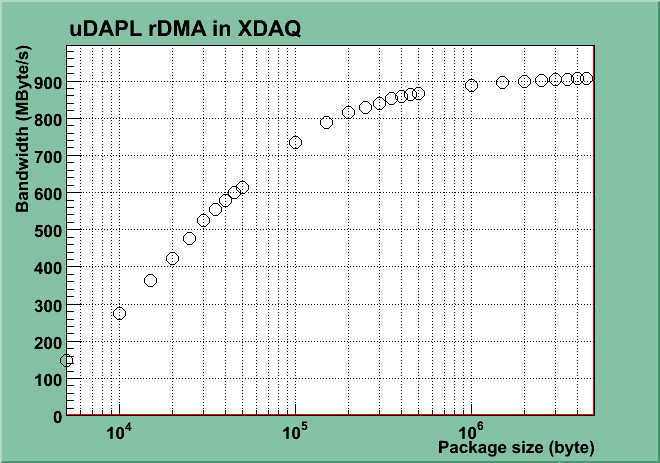
\includegraphics[angle=0,width=.8\textwidth]
{RoundtripRDMA.png}
\caption{Bandwidth versus package size from roundtrip benchmark of
plain rDMA within the XDAQ framework}
\label{fig:rdmaroundtripbw}
\end{figure}

For the benchmark, 
the sender {\em ConfigureAction()} opens a remote DMA connection
to the receiver application. A thread in the sender 
application then transfers packages with increasing size and
measures bandwidth and transfer time.
From these measurements, one gets values as shown in 
Fig.~\ref{fig:rdmaroundtripbw}.
The corresponding parameters from the fit (eq. \ref{eq-taup})
are: 

\centerline{$\tau_{0}=25~\mu\mbox{s}$ and $B_{P\to\infty} = 955~\mbox{MByte/s}$.} 

Compared with table \ref{tab-ether-ib-tcp}, this is already
a big improvement. However, the performance of the plain uDAPL tests
(section \ref{uDAPL-testapp}) was not achieved, since
the set up for the uDAPL buffer queues was not optimized here.
Moreover, for a real data transfer application in XDAQ, the
I2O messaging should be used. Thus the development of a
peer transport uDAPL library was a strong requirement.


\subsection{PeerTransportDAPL implementation}
\label{ptDAPL-Imp}

%We did it! Explain how, only show last implementation, brief form.
%Maybe UML class diagram here?
Our implementation of a peer transport 
library for uDAPL was originally based on the architecture of
the existing library for tcp/ip {\em pt/tcp} \cite{XDAQ-wiki}. 
Most of the classes and their relationship were at first just adopted and
renamed from namespace ``tcp'' to namespace ``ptdapl''.
The usage of tcp/ip {\em socket} calls was replaced by the
corresponding functionality as provided by the uDAPL library.
Actually, our general uDAPL interface class {\em TBasic}
(\ref{uDAPL-cpp}) was embedded into the {\em ptdapl::Channel} class.






Figure (\ref{fig:ptdaplclasses}) shows the UML class diagram overview for 
the final implementation. 
In the following, we describe the ptdapl
classes in detail.


\begin{description}

\item[PeerTransportDAPL:] The owner of {\em PeerTransportSender} and 
{\em PeerTransportReceiver}. 
These are registered in the general {\em PeerTransportAgent} as available 
from pt framework. Offers web and cgi interface for interactive configuration. 
Some connection parameters for uDAPL may be 
set in the configuration file. These are passed via peer 
transport sender/receiver instances to the channels that use them.  
Method {\tt reset()} will apply changes to sender and receiver components. 

\item[ptdapl::Channel:] This is the baseclass of {\em ptdapl::Transmitter} and 
{\em ptdapl::ReceiverLoop}. Aggregates the {\em TBasic} class as interface to the 
uDAPL functionality. 

\end{description}
   
\begin{figure}[htb]
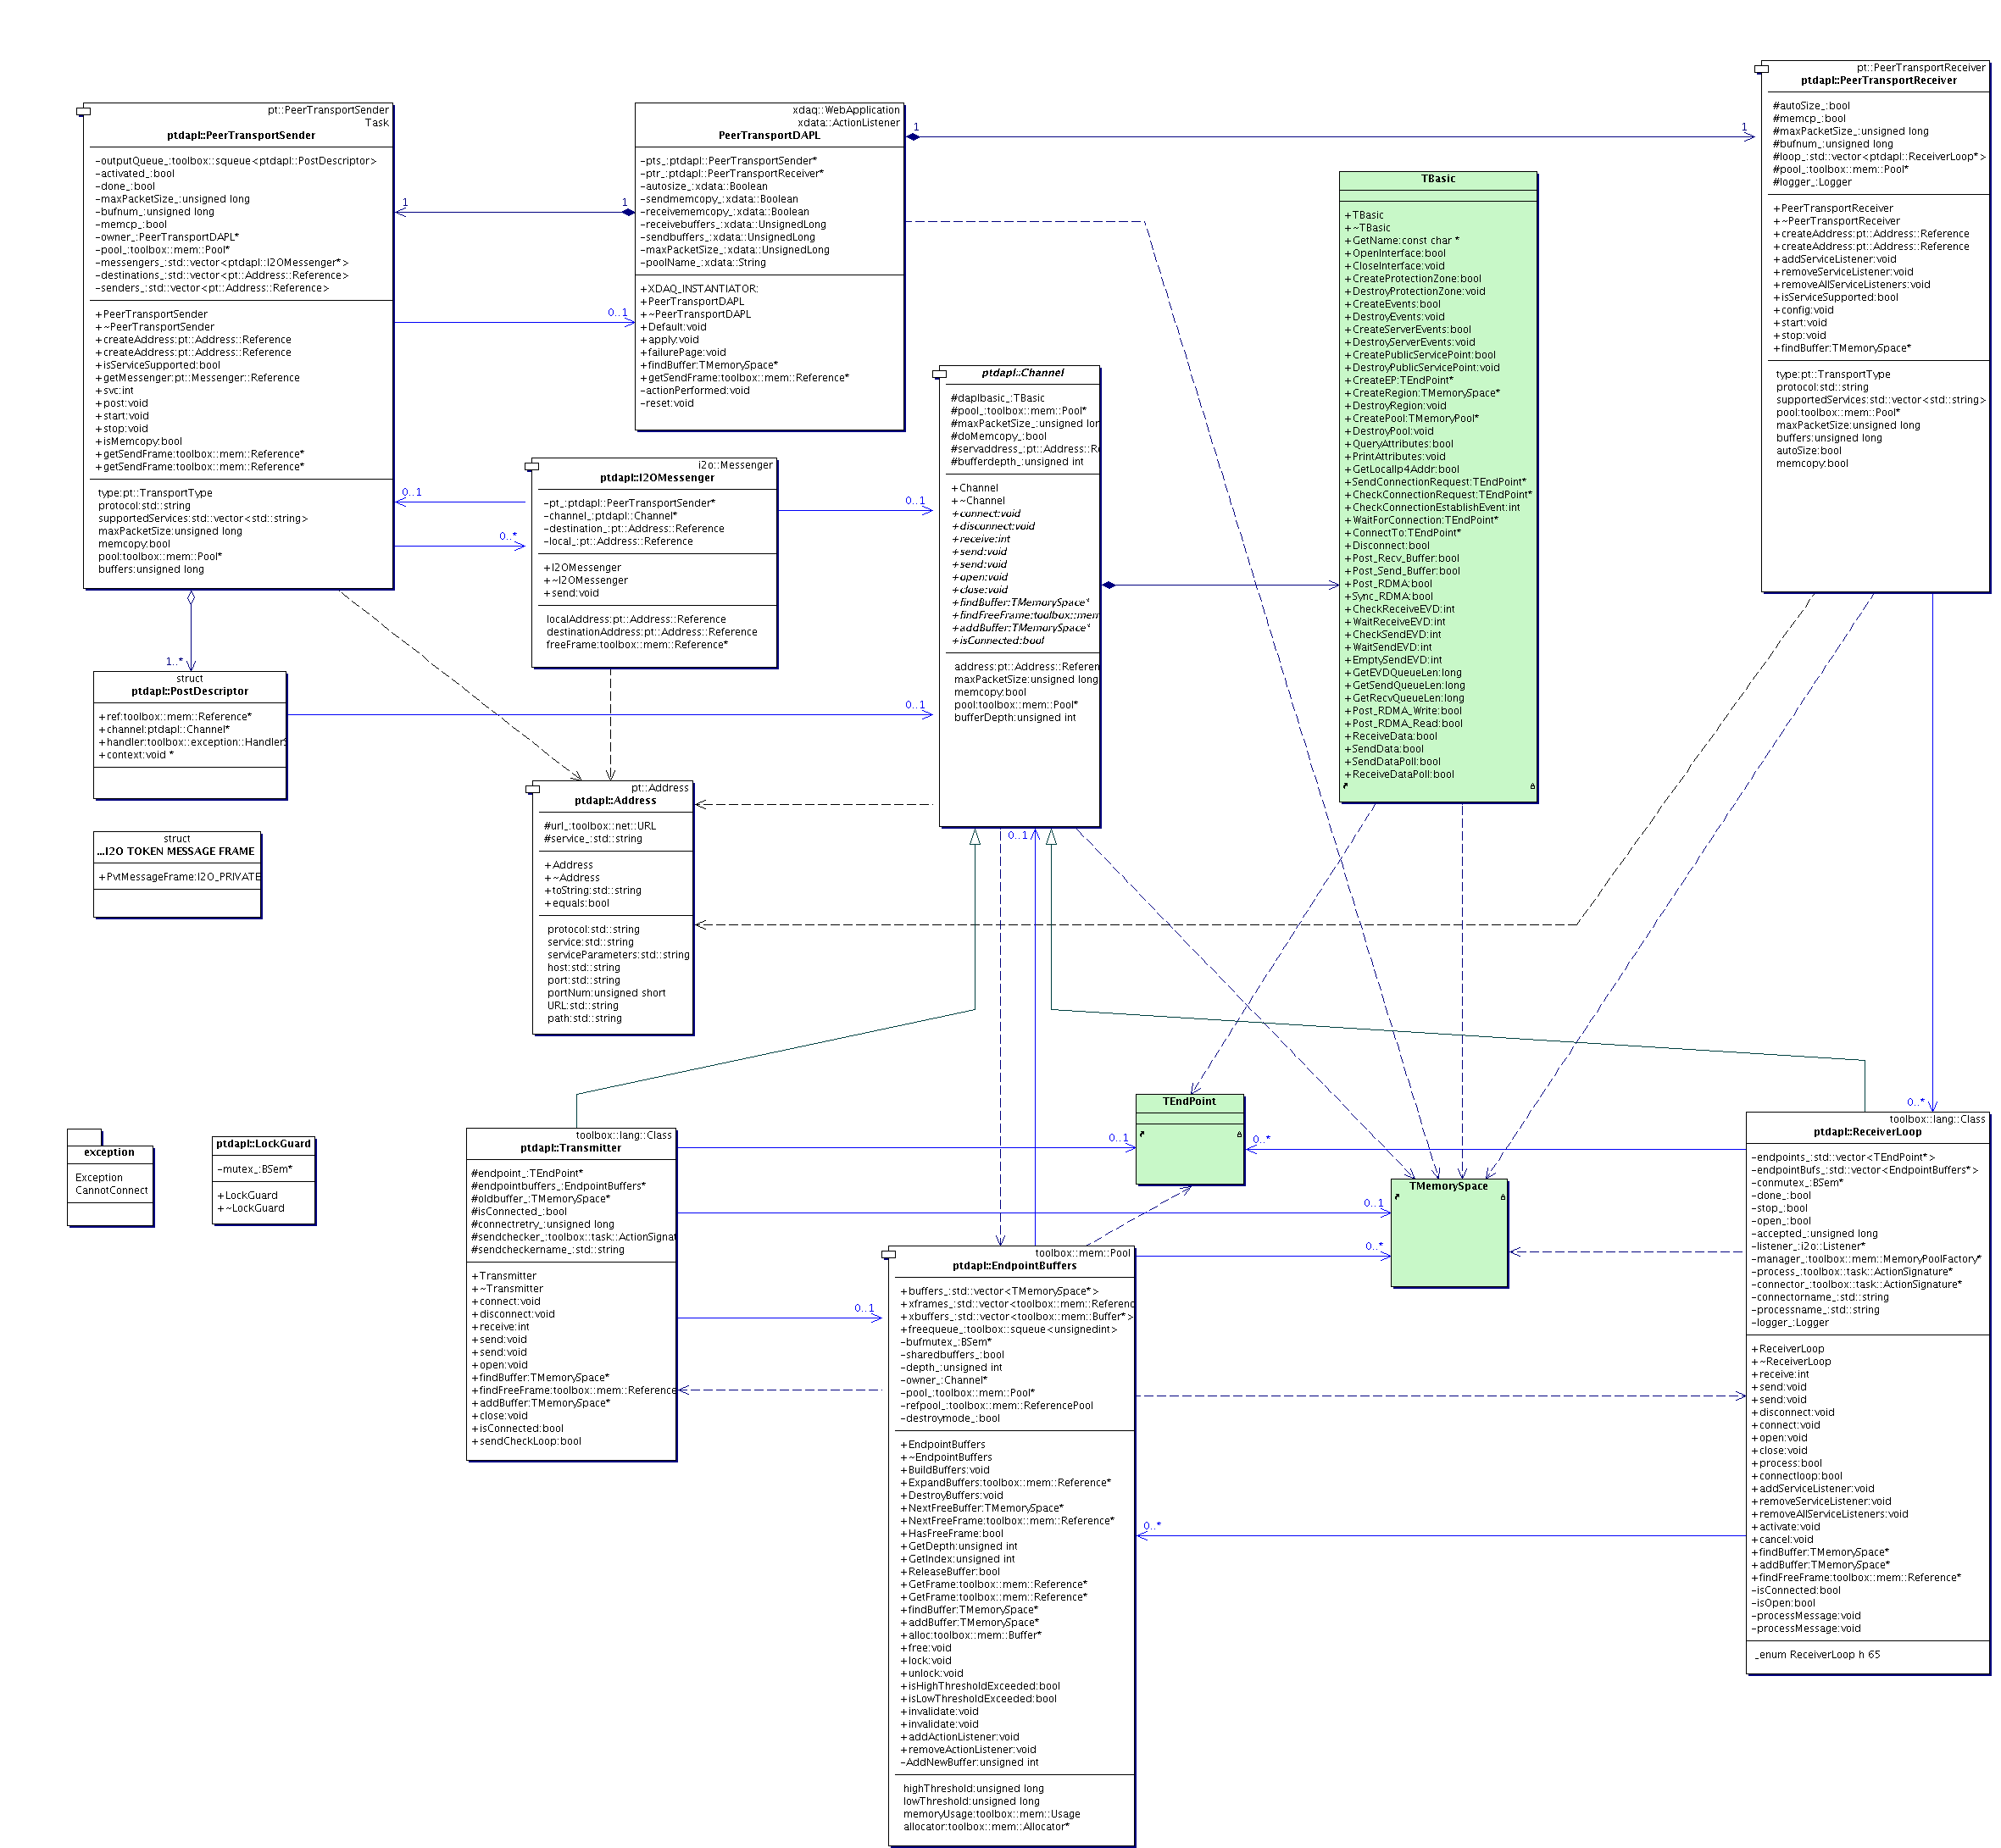
\includegraphics[angle=90,width=1.0\textwidth, height=1.0\textheight]
{ptdapl.png}
\caption{{\em PtDAPLClasses} Class diagram of the peer transport DAPL implementation for XDAQ}
\label{fig:ptdaplclasses}
\end{figure}



\begin{description}
\item[ptdapl::PeerTransportSender:] The sender of data.
\begin{compactitem}[$\bullet$]
      \item Method {\tt svc()} runs in a waiting workloop 
(as background thread). It waits for the output queue that contains 
the {\em ptdapl::PostDescriptor} objects. The memory frames as 
defined in this descriptor are transferred by method {\tt send()}  
of corresponding {\em ptdapl::Transmitter} 
(also referenced in post descriptor structure).
      \item Method {\tt post()} is used from the outside 
client to generate a new {\em PostDescriptor} in the output queue.
      \item {\tt getMessenger()} is a factory method for the appropriate 
messenger that shall manage the sending. 
This is finally used from the application context messenger cache. 
\end{compactitem}

 \item[ptdapl::Transmitter:] The sending client. Methods {\tt connect()}, 
{\tt send()}, implemented with \newline
{\tt TBasic::SendConnectionRequest()} 
and {\tt TBasic::PostSendBuffer()}, resp.



\item[ptdapl::I2OMessenger:] Manages the sending functionality.
The owner of the {\em ptdapl::Transmitter}.

\begin{compactitem}[$\bullet$]
\item is used by 
{\tt xdaq::ApplicationContextImpl::postFrame()}. 
This is the recommended user interface to send i2o frames. 
Application context instance has {\em messengerCache} 
which keeps the messengers by originator and destination tags 
({\em xdaq::ApplicationDescriptor}s of {\tt postFrame()} 
arguments). For each pair of originator and destination 
there is one messenger. If a messenger for a 
pair does not exist, the messenger cache will create it, 
using the build method {\tt getMessenger()} of {\em PeerTransportSender}.

\item method {\tt send()} internally calls 
the {\tt post()} of the corresponding {\em PeerTransportSender} 
that created it.

\item method {\tt createAddress()} generates address references 
for sender and receiver nodes from url/service.



\end{compactitem}

\item[ptdapl::Address:] Keeps connection address parameters. 
Added method {\tt getPortNum()} to get number of connection port 
by value. This parameter is used here as port number 
for the uDAPL connection.

\end{description}

%\clearpage

\begin{description}

\item[ptdapl::PeerTransportReceiver:] The receiver of data on each node. 
     Has vector of {\em ptdapl::ReceiverLoop} objects; these are activated 
in method {\tt start()} and canceled in {\tt stop()}. Method 
{\tt config()} generates new {\em ReceiverLoop} object in this vector for 
each receiver node address (network endpoint). 
Additionally, baseclass {\em pt:PeerTransportReceiver} has
a map of {\em i2o:Listener} objects by name.
The listener of name "i2o" is used for all {\em ptdapl::ReceiverLoop} 
objects which get its reference during {\tt config()}.


 \item[ptdapl::ReceiverLoop:] The receiving server. Has two working threads:
\begin{compactitem}[$\bullet$]
\item Thread {\tt connectloop()} establishes the connection:
it creates an uDAPL endpoint whenever requested from a new sender client. 
The {\em ReceiverLoop} instance may have 
many endpoints, each connected to another remote {\em Transmitter}. 

\item Thread {\tt process()} does the receiving.  
It waits for an uDAPL receive event from any existing endpoint.
On receive, the incoming endpoint receive buffer is  
passed to the {\em i2o::Listener} which forwards the message to
the destination callback function.
\end{compactitem}

\item [i2o::Listener:] Handles incoming i2o messages (frames). This
is a general messaging framework class, not part of the {\em ptdapl} 
library. 
\begin{compactitem}[$\bullet$]
\item The implementation of listener is done in subclass 
{\em i2o::utils::Dispatcher}. This dispatcher is created and 
added to the peer transport agent in the constructor of the 
XDAQ {\em Executive} class. There are also other dispatchers for {\em xgi} and {\em SOAP}.

\item   Method {\tt processIncomingMessage(msg)} does the actual work: 
the I2O message contains target and function ids. The dispatcher will find 
the {\em i2o::MethodSignature} reference by these ids from the application. 
With  {\tt i2o::MethodSignature::invoke(msg)} the I2O message {\tt msg} 
is passed over to the callback method, as registered in the
user code by {\tt i2o::bind()}.  
\end{compactitem}


\end{description}

\clearpage

{\bf During several development cycles with continuous 
improvements, additional classes and functionality dedicated
to uDAPL transport were introduced: }

\begin{description}

\item [ptdapl::EndpointBuffers:] New class that manages
the uDAPL send and receive buffers of a connection
embedded into regular XDAQ memory frames.

\begin{compactitem}[$\bullet$]

\item Is owned by a {\em Channel} both in sender and receiver
implementation:
The {\em Transmitter} has one {\em EndpointBuffers} pool, whereas
a {\em ReceiverLoop} holds one {\em EndpointBuffers} object for each
incoming endpoint.

\item Pool for XDAQ memory
frames that internally wrap already assigned uDAPL send and receive
buffers, to minimize copying between XDAQ and uDAPL memory. 
It holds parallel vectors of uDAPL buffers, 
XDAQ frames, and their {\em toolbox::mem::Reference}s.  



\item Subclass of the XDAQ memory pool 
{\em toolbox::mem::Pool}. Overwrites standard 
methods {\tt alloc}, {\tt release}. When application
does a {\tt release()} on a XDAQ memory frame from this pool
(after processing the received package),
it will not free the allocated memory, but will push the
buffer index into a queue of free buffers, and refresh the
XDAQ reference. Similarly, after having completed the send of a frame,
it is just marked as ``free'' by queueing its index.
So in both use cases, the buffer is immediately available again
without performance loss due to 
re-allocation and registration as uDAPL endpoint buffer.


\item  Method {\tt findBuffer(toolbox::mem:Reference*)}:   
checks if any memory reference belongs to an already created 
uDAPL input or output buffer. In this case, the buffer can be send
without first copying the contents from XDAQ frame to uDAPL buffer.
The owner class {\em Channel} also offers 
a virtual {\tt findBuffer()}, which is implemented for {\em Transmitter} 
and {\em ReceiverLoop}, scanning all contained {\em EndpointBuffers}.
From outside, the {\tt findBuffer()} method is
accessible in the {\em PeerTransportReceiver} and
{\em PeerTransportDAPL} aggregations, too.


\item Method {\tt addBuffer(toolbox::mem:Reference*)}: adds
a new uDAPL endpoint buffer that uses an existing XDAQ memory frame.
Especially useful for
the {\em RoundTrip} application, when a buffer from the receiver endpoint 
can also be assigned to the sender endpoint.  
On the next roundtrip cycle, this reference will be found as
existing send buffer and transferred 
without any data copying.

\end{compactitem}
\medskip

\item [ptdapl::Transmitter:] direct buffer sending and 
asynchronous releasing:
\begin{compactitem}[$\bullet$]

\item new  method {\tt send(TMemorySpace * dbuf, int len)}.
Will post existing uDAPL buffer directly; old method 
{\tt send(void* buf, int len)} will still perform {\tt memcpy} into a 
buffer of  internal {\em EndpointBuffers} pool before sending.
In the final implementation, both methods will return before 
send completion was acknowledged from uDAPL. After the send call, the
{\em PeerTransportSender} will not {\tt release()} the frame itself, 
but this is done asynchronously by a second thread. 

\item new thread (workloop) {\tt sendCheckLoop()}. 
Waits for any send complete event from the uDAPL interface. Required
to add appropriate implementation in 
basic uDAPL interface \newline {\tt TBasic::WaitSendEVD()}. 
On send complete event, the thread will get the buffer reference from the
posted uDAPL cookie and will  {\em release()} this frame.
{\em Transmitter} had to be changed to inherit from
{\em toolbox::lang::Class} in order to run a method as XDAQ workloop. 

\end{compactitem}


\item [PeerTransportDAPL:]
\label{ptdaplgetsendframe}
additional method: 
{\tt getSendFrame(context, from, to)}: 
Returns memory reference of next free send buffer by descriptors of sender 
("from") and receiver ("to") application. Syntax is similar to the 
{\tt ApplicationContext::postFrame(...)} as called by the 
user code for sending. Thus, the user code may directly get a
reference to an uDAPL send buffer from the peer transport implementation.
This is useful to avoid another copying of data, since the user may
directly modify the assigned uDAPL memory contents before posting it.

However, to use this feature, downcasting of the application pointer 
to {\em PeerTransportDAPL} is necessary in user code. 
This will break the XDAQ philosopy of modularity 
and the decoupling between application and peer transport though. 
Actually, the {\em MyRoundTrip} application 
(section \ref{ptDAPL-RoundTrip}) had to be
modified in a way that the {\em PeerTransportDAPL} instance was
retrieved on configuration time via its id number  
from the XDAQ application registry .
Therefore, the XML configuration 
parameter {\em peerTransportID} was introduced to the 
{\em MyRoundTrip} set up.


Finally, the 
configuration parameters for the {\em PeerTransportDAPL}
allow to
specify the number of send and receive buffers in the pool, and
to switch on/off the {\tt memcpy} functionality for sending
and receiving. 

\end{description}







\subsection{RoundTrip with PeerTransportDAPL}
\label{ptDAPL-RoundTrip}
%Roundtrip, etc. main-test.pdf
\begin{figure}[htb]
\centering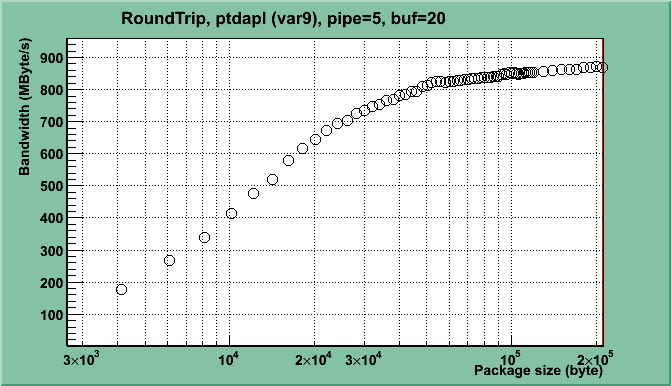
\includegraphics[angle=0,width=.8\textwidth]
{RoundtripPTDAPL.png}
\caption{Bandwidth versus package size from roundtrip benchmark of
I2O over {\em PeerTransportDAPL} (var.~9)}
\label{fig:ptdaplroundtripbw}
\end{figure}


In the course of the development of the {\em PeerTransportDAPL},
the {\em MyRoundTrip} benchmark
(section \ref{RoundTripBasics}) was applied to check the
performance and figure out implementation disadvantages.
The roundtrip application was mostly unchanged to the tcp/ip
peer transport measurements (section \ref{RoundTripTestTCP}).
For the final implementations, however, accessability to the
{\em PeerTransportDAPL} was introduced to {\em MyRoundTrip}, 
allowing direct writing of the user code 
into the preassigned uDAPL send buffers 
(section \ref{ptdaplgetsendframe}).

The following are the results of this best optimized
{\em PeerTransportDAPL} implementation (variant 9).
Figure \ref{fig:ptdaplroundtripbw} shows bandwidth versus package size
for the roundtrip of 5 initial packages and 20 receive buffers. The
maximum number of uDAPL buffers was set to 32 here.


 Figure 
\ref{fig:ptdaplroundtriptau} plots the corresponding transport times 
$\tau(P)$.
From the fit (eq. \ref{eq-taup}) to this curve,
we get the parameters of merit:

\centerline{$\tau_{0}=5.5~\mu\mbox{s}$  and $B_{P\to\infty} = 935~\mbox{MByte/s}$.} 

This is obiously better than the peer transport via tcp, and
reaches almost the speed of the plain uDAPL tests.

\begin{figure}[htb]
\centering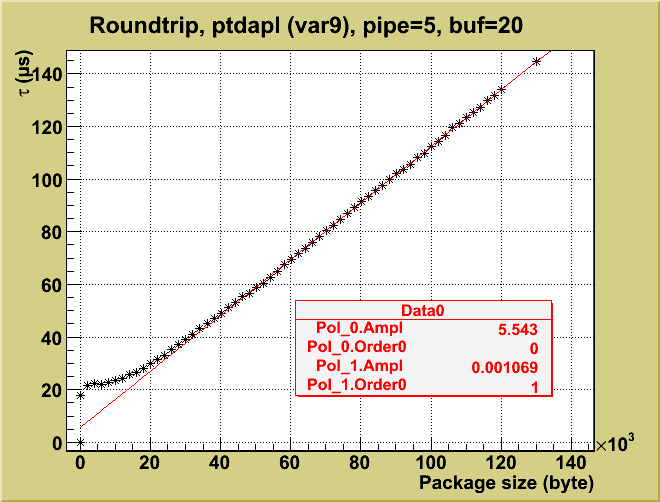
\includegraphics[angle=0,width=.8\textwidth]
{RoundtripPTDAPL-tau.png}
\caption{Transport time versus package size from roundtrip benchmark of
I2O over {\em PeerTransportDAPL} (var.~9). 
Red line shows fit of (eq. \ref{eq-taup}) at linear part of the curve.}
\label{fig:ptdaplroundtriptau}
\end{figure}


However, the {\em real} minimum latency $\tau_{min}\simeq 20~\mu\mbox{s}$ 
is larger than the fitted characteristic $\tau_{0}\simeq 5~\mu\mbox{s}$.
For small packages, the transport is just limited 
by the XDAQ framework latency that is invariant with package size. 
The fitted equation (\ref{eq-taup}) is valid 
for big packages only, where the uDAPL maximum speed rules the
transfer time. Since this peer transport implementation uses two
threads for asynchronous posting and releasing of the send buffers,
the overall transport time shows the maximum of both 
effects only: If uDAPL transfer is faster (small packages), 
the latency to invoke the {\em postFrame} and to 
get the next free buffer from the pool 
is the limit. Otherwise (big packages), the XDAQ buffer management 
is always ready before the network data transfer has completed.

In contrast to this, a previous implementation of {\em PeerTransportDAPL}
(variant 8) with only one sender thread showed a curve $\tau(P)$ that
was the {\em sum} of both effects over the complete range.
This was due to the fact that the sender thread had to 
wait for the uDAPL transfer complete event of each frame before
it could process the next send frame. Thus, the linear part of the 
curve was shifted upwards by the constant offset $\tau_{min}\simeq 20~\mu\mbox{s}$.






\clearpage
\subsection{Sender-Receiver with PeerTransportDAPL}
\label{ptDAPL-SendRec}
%Roundtrip, etc. main-test.pdf
Although the RoundTrip is useful for benchmarking, 
it is different from the future
applications for the DAQ system. Here the data is send by one
application and received by another application. For such a set up,
the shared buffering for sender and receiver endpoints, as implemented
for the  {\em PeerTransportDAPL}, will not
yield any performance gain. Instead, the management of the buffer pool 
becomes crucial for the latency.


To measure such a situation, we implemented a pure
sender application as class {\em MyDataSource}, and a mere
receiver as {\em MyDataDrain}. Both have initially been developed as
modifications of the {\em MyRoundTrip} class: 

\begin{description}
\item [MyDataSource:]  Once enabled by the controlling state machine,
the {\em Benchmark()} workloop (thread) 
posts frames to the receiver {\em MyDataDrain}. 
The sending pipeline loop of {\em MyRoundTrip} is still used.
Integer numbers are written to the I2O data field,
corresponding to the pipeline position. 
The performancemeter is called at the beginning of each pipeline circle. 
When the performancemeter has reached its number of samples, 
the package size is increased (as in {\tt MyRoundTrip::token()}). 

The new send frames are directly requested from peer transport DAPL instance
(section \ref{ptdaplgetsendframe}). If the peer transport instance 
is not found (e.g. because of a wrong application id 
number in the setup file),  {\em MyDataSource} will allocate send 
frames from the standard 
XDAQ memory pool\footnote{ 
In this case, a problematic polling behaviour was observed, 
because the standard  memory pool soon runs out of preallocated 
buffers.  Then the {\tt Benchmark()} function has to react on the 
exception  thrown and retries to allocate a new frame. 
This will drop the performance by a factor of 2.}.
 

\item [MyDataDrain:] Reacts on the received  I2O packages in 
{\tt token()} callback only.  
Here, with knowledge of the sender pipeline length (by configuration file), 
it invokes the performancemeter for each leading packet of the pipe cycle. 
The contents of each I2O frame (pipe entry number) 
are read and may be checked for data integrity.

\end{description} 
 



As in the RoundTrip, both classes provide 
a web interface to display the benchmark results.

The independent performancemeter measurements on sender and receiver
applications yielded the same results. This should be expected for
``conservation of data current'' reasons. Moreover, also for several
senders and receivers (``one to all'' , see \ref{ptDAPL-SendMultRec}; 
``all to one'', see \ref{ptDAPL-MultSendRec}), the sum of
sender and receiver latencies was matching.
Therefore, for the ``one to one'' set-up, 
we just evaluate the data source performance.


%\clearpage

\begin{figure}[htb]
\centering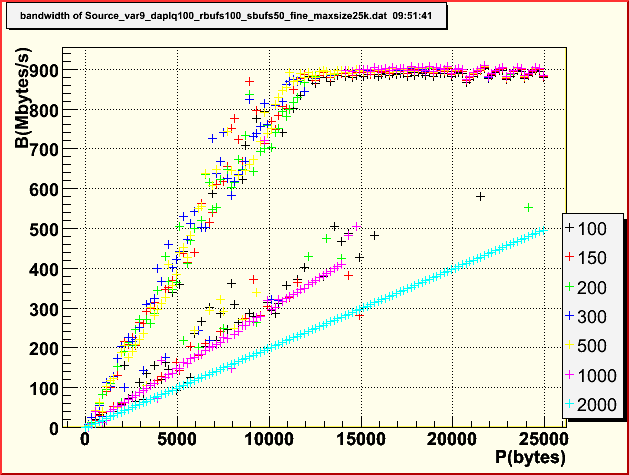
\includegraphics[angle=0,width=.82\textwidth]
{var9_q100_rbufs_bw.png}
\caption{Bandwidth versus package size from 1 to 1 data transfer using
{\em PeerTransportDAPL} (var.~9). $N_{send}=50$, $N_{q}=100$, }
\label{fig:ptdaplsourcedrainbw}
\end{figure}

\begin{figure}[htb]
\centering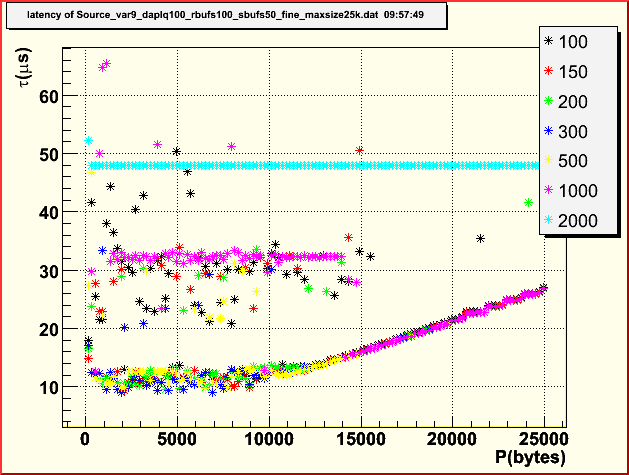
\includegraphics[angle=0,width=.82\textwidth]
{var9_q100_rbufs_lat.png}
\caption{Transfer time versus package size from 1 to 1 data transfer using
{\em PeerTransportDAPL} (var.~9). $N_{send}=50$, $N_{q}=100$, }
\label{fig:ptdaplsourcedraintau}
\end{figure}

%\clearpage


Several measurements were done under variaton of the send
and receive buffer numbers.

Besides the number of buffers in the endpoint pools
$N_{send}$ and  $N_{rcv}$,
the predefined maximum uDAPL endpoint buffer queue length
$N_{q}$ is crucial. It is not possible to post more buffers 
than $N_{q}$ to an endpoint simultaneously, thus limiting the effective
usable buffer number of the {\em EndpointBuffers} pool.
By default, half of
the existing {\em EndpointBuffers} frames are assigned
to each endpoint in advance, up to $N_{q}$.

$N_{q}$ is set up on compile time  of the uDAPL wrapper library.
While we used $N_{q}=32$ for the initial roundtrip benchmarks, we
increased it to $N_{q}=100$ for the sender-receiver measurements.

It turned out that the performance improved with increasing
number of receive buffers, up to $N_{rcv}\simeq 500$. Then, it
drops again, probably due to the overhead of searching the
next free buffer in the pool (values for $N_{q}=100$).
Similar was found concerning the send buffers.

Figure (\ref{fig:ptdaplsourcedrainbw}) shows the bandwidth versus
the frame size for these measurements; figure 
(\ref{fig:ptdaplsourcedraintau}) the corresponding transport time.



Observations:
\begin{compactitem}

\item As for the Roundtrip, the $B(P)$ characteristics has 2
different domains:
\begin{enumerate}
\item For smaller packages ($< 10$~kByte), the bandwidth increases 
approximately linear with package size, i.e. the transport time per package 
is constant. Here the transfer is limited by the xdaq buffer management, 
because the uDAPL transfer is faster than the 
finding/releasing of the buffers. Obviously, in this domain
some points show big fluctuations from the ``ideal curve''.

\item For bigger packages ($>10$~kByte), the bandwidth nearly 
saturates very fast to the theoretical transfer limit. 
Here the transport is limited by the uDAPL interface, 
Even here we see some points with big fluctuations, 
but the overall line is more straight than in domain 1 

\end{enumerate}

\item For few receive buffers (less than uDAPL queue length), 
the linear increase region of $\tau$ starts later; 
the "constant $\tau$  region" has more fluctuations. 
Here the uDAPL receive queue is not fully used, 
since only half of XDAQ buffers are posted in advance; 
full uDAPL queing only for  $N_{rcv}> 200$ .

\item For $N_{rcv} \geq 1000$, there is a almost a ``state transition''
step between the constant latency region and the linear latency 
region. At $P\simeq 14$~kByte, the transfer time drops almost
about $20~\mu$s. This corresponds with a very steep edge 
in the bandwidth characteristics. As an explanation,
one can think of an extra delay when suddenly one of the
involved threads has to wait for a synchronizing signal.
These can be the sender and cleanup threads (sender application),
and here most likely the receiverloop thread and the I2O
callback thread (receiver application).

For big packages, the receiverloop thread (or sender, respectively) 
never has to wait for the queue of next free buffers, 
because there is always a
free buffer ready in the queue before uDAPL transfer has finished.

At a certain package size (minimum of linear $\tau$ region), both
threads are ``synchronized'' - for uDAPL it takes the same time to receive
(send, resp.) a package as for XDAQ to release another frame 
and to handle the memory pool management. 
If the package size decreases just a little bit, uDAPL transfer is completed
before the queue of free
buffers has a new buffer ready. Then, the receiver (sender, resp.) thread
will go into a thread condition {\em wait()} when trying to get the next
queue entry. It will continue no sooner than the other thread pushes
another frame into the queue, thus waking up the  receiver (sender,resp.)
by a condition signal.
The observed latency difference at the edge might correspond to the time that 
is required for the queue to schedule this signal, 
in comparison to a plain {\tt pop()} of an existing queue element.

 

\item For big XDAQ receive buffer pool, the constant latency is large 
( $\tau_{min} > 32\mu\mbox{s}$). This can be explained by an increasing 
average search time for the next free buffer in the xdaq mempool.

\item The fits to the latency curve (eq. \ref{eq-taup}) gives the
parameter 
$ \tau_{0} < 0.1~\mu\mbox{s}$, 
i.e. the linear fit almost crosses origin. 
The slope yields $c\approx 1.07~\mu\mbox{s/kByte} $, thus a bandwidth 
limit of $B_{max}\approx 935~\mbox{MByte/s} $ is achieved.

\end{compactitem}




\subsection{One sender for multipe receivers with PeerTransportDAPL}
\label{ptDAPL-SendMultRec}

A DAQ application will most possible not transfer the data 
in between just 2 nodes, but each sender node has to post
parts of the event to many different builder nodes.

\begin{figure}[htb]
\centering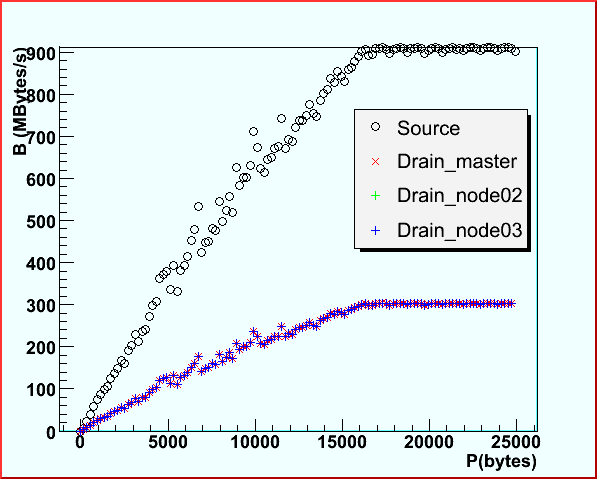
\includegraphics[angle=0,width=.8\textwidth]
{var9_1to3_bw.png}
\caption{Bandwidth versus package size from 1 to 3 data transfer using
{\em PeerTransportDAPL} (var.~9). $N_{send}=50$, $N_{rcv}=300$, $N_{q}=100$ }
\label{fig:ptdapl123bw}
\end{figure}

To test such a situation, the test set up with slightly modified
sender application was as follows:

\begin{compactitem}
\item {\em MyDataSource} application will check from {\em destinationID}  
number where to send the data. 
In {\tt ConfigureAction()}, the application descriptors with 
matching {\em tid}s will be found by iteration over the {\em ContextTable}; 
if the target application exists as described in configuration file, 
it will be put into {\em std::vector} of destinations. 

\item The {\tt Benchmark()} sender thread will distribute 
data in ``round robin'' fashion to all known destinations. 
Each receiver application will get a complete output pipeline 
before the next receiver is served. 

\item If the {\em tid} is unknown in the context, an exception will 
indicate a warning 
(e.g. if any of the known nodes has only a sender, but no receiver). 

\item Performance measurements are done independently in sender and all receivers. 

\end{compactitem}



A typical result is plotted in figure \ref{fig:ptdapl123bw}.
Observations:
 \begin{compactitem}
\item The sender reaches the same performance as in the one-to-one setup 
before (latency and bandwidth limit)
 
\item Each receiver gets one third of sender bandwidth, as expected.
 
\item The values of all 3 receivers match very exactly (bandwidth, latency). 
All curves show the same structures/deviatons from the ``expected line''. 
Maybe this stems from overall fluctuations of the network or the switch, 
since it  seems not to be related to the individual load of the
receiver machines 
 \end{compactitem}

\clearpage
\subsection{Multiple senders for one receivers with PeerTransportDAPL}
\label{ptDAPL-MultSendRec}

Vice versa, 
performance tests were done with several sender applications to address
one receiver. Here it shows up if the {\em ReceiverLoop} organization
of the peer transport works well for more than one incoming endpoint.
The application set up was the same as described in section (\ref{ptDAPL-SendMultRec})





\begin{figure}[htb]
\centering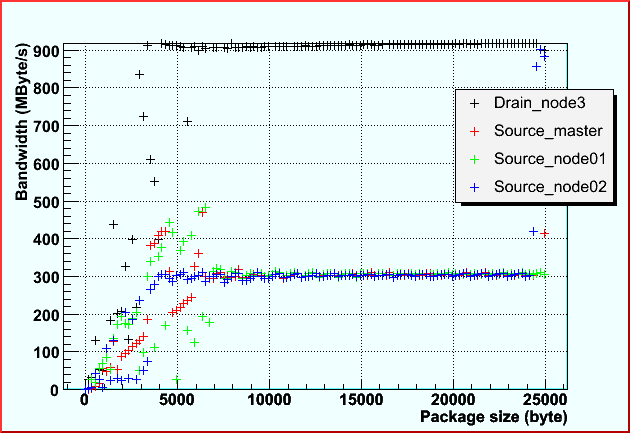
\includegraphics[angle=0,width=.8\textwidth]
{var9_3to1_bw.png}
\caption{Bandwidth versus package size from 3 to 1 data transfer using
{\em PeerTransportDAPL} (var.~9).  $N_{send}=50$, $N_{rcv}=300$, $N_{q}=100$}
\label{fig:ptdapl321bw}
\end{figure}

Figure \ref{fig:ptdapl321bw} illustrates some results.
Especially for small package sizes, the multiple senders  
show more differences in bandwidth than in the opposite case 
(\ref{ptDAPL-SendMultRec}) the multiple receivers.
Still the sum of all sender bandwidths yields the receiver 
bandwidth very exactly. Above a threshold of $P\simeq 8$~kB,
each senders contributes about a third of the receiver bandwidth.


